\chapter{Analyse de la méthode JFNK dans CEDRE}

  \paragraph{}
  In a previous chapter, we identified some methods from the literature that we wanted to use in our solver CEDRE, and some others from CEDRE that we wanted to improve.
  In another chapter, we discussed the practical implementation of said methods in the solver.
  The goal of this chapter is now to test those methods on several applications to comment on the choices we made.
  We need to define test cases that represent well enough target applications so we can comment on the performances of our choices.


  \section{Comparaison entre la matrice jacobienne explicite et la formulation sans matrice}

    \paragraph{}
    From our analysis and implementation, the main addition to the solver is the Jacobian Free Newton--Krylov method, and in particular the matrix-free approach.
    In this part, we will then compare two methods: the traditional method and the new one that uses the matrix-free approach.
    As we are interested in implicit time integration, we will use the implicit Euler method, for reasons previously discussed.
    The traditional method linearises the equation that the implicit Euler method produces, approximates the Jacobian matrix using the Jacobian matrix of the corresponding first-order scheme, and then solves the linear system with the Krylov subspace method GMRES.
    As we want to understand the impact of a better Jacobian matrix, we are only going to change how it is computed.
    The new method will then work in a similar way, except the matrix used in the linear solver is not actually computed, but the matrix-vector products are approximated using equation (\ref{eq:matrix_free}).


    \subsection{Turbulent transonic airfoil}

      \subsubsection{Definition of the test case}


        \PS{TODO: sûr de aoa et Re ?}

        \paragraph{}
        Our first application is a typical aerodynamics test case.
        It is a 2D simulation of the flow around an RAE 2822 wing profile.
        The only fluid is standard air.
        The Mach number is taken equal to 0.75, the chord is equal to $1\si{\meter}$, the angle of attack is $0\si{\degree}$ and we use the atmospheric conditions at 10km.
        This gives a Reynolds number of \num{6.3e6}.

        \paragraph{}
        We decided to use this first test case for multiple reasons.
        Firstly, it is a simple case in the field of computational fluid dynamics.
        It is a standard aerodynamics case, with a small mesh in comparison to many other 3D cases.
        This allows us to test out methods inexpensively.
        Secondly, this case belongs to the tutorial suite of our solver.
        It means that it is already well mastered by the team.
        Thirdly, even if it is only a standard aerodynamics case it still has some stiff features, such as turbulence modelling and a shock.
        Finally, it is a standard test case for turbulence modelling validation.
        Therefore there are many references in the literature using this case. \PS{LES DONNER !}
        Even if this thesis aims at multiphysics, it is often good to start slow, and that is what we are doing with this test case.

        \paragraph{}
        The mesh used for this simulation is an unstructured hybrid mesh made of triangles and quadrangles \PS{c'est bien ça ?}.
        Parts of it can be seen in figure \ref{fig:rae_mesh}.
        Cell sizes range from $2.5\si{\meter}$ far from the airfoil and $100\si{\micro\meter}$ at the wall.
        At the wall, there is a C-shaped layer of regular cells.
        This helps better capture boundary layer effects near the profile and the \PS{pas vraiment lâcher tourbillonnaire}.
        Also, at those conditions, a shock is expected to develop on the upper part \PS{extrados ?}.
        Special treatment such as refinement was applied to the mesh at the expected shock location.

        \begin{figure}
          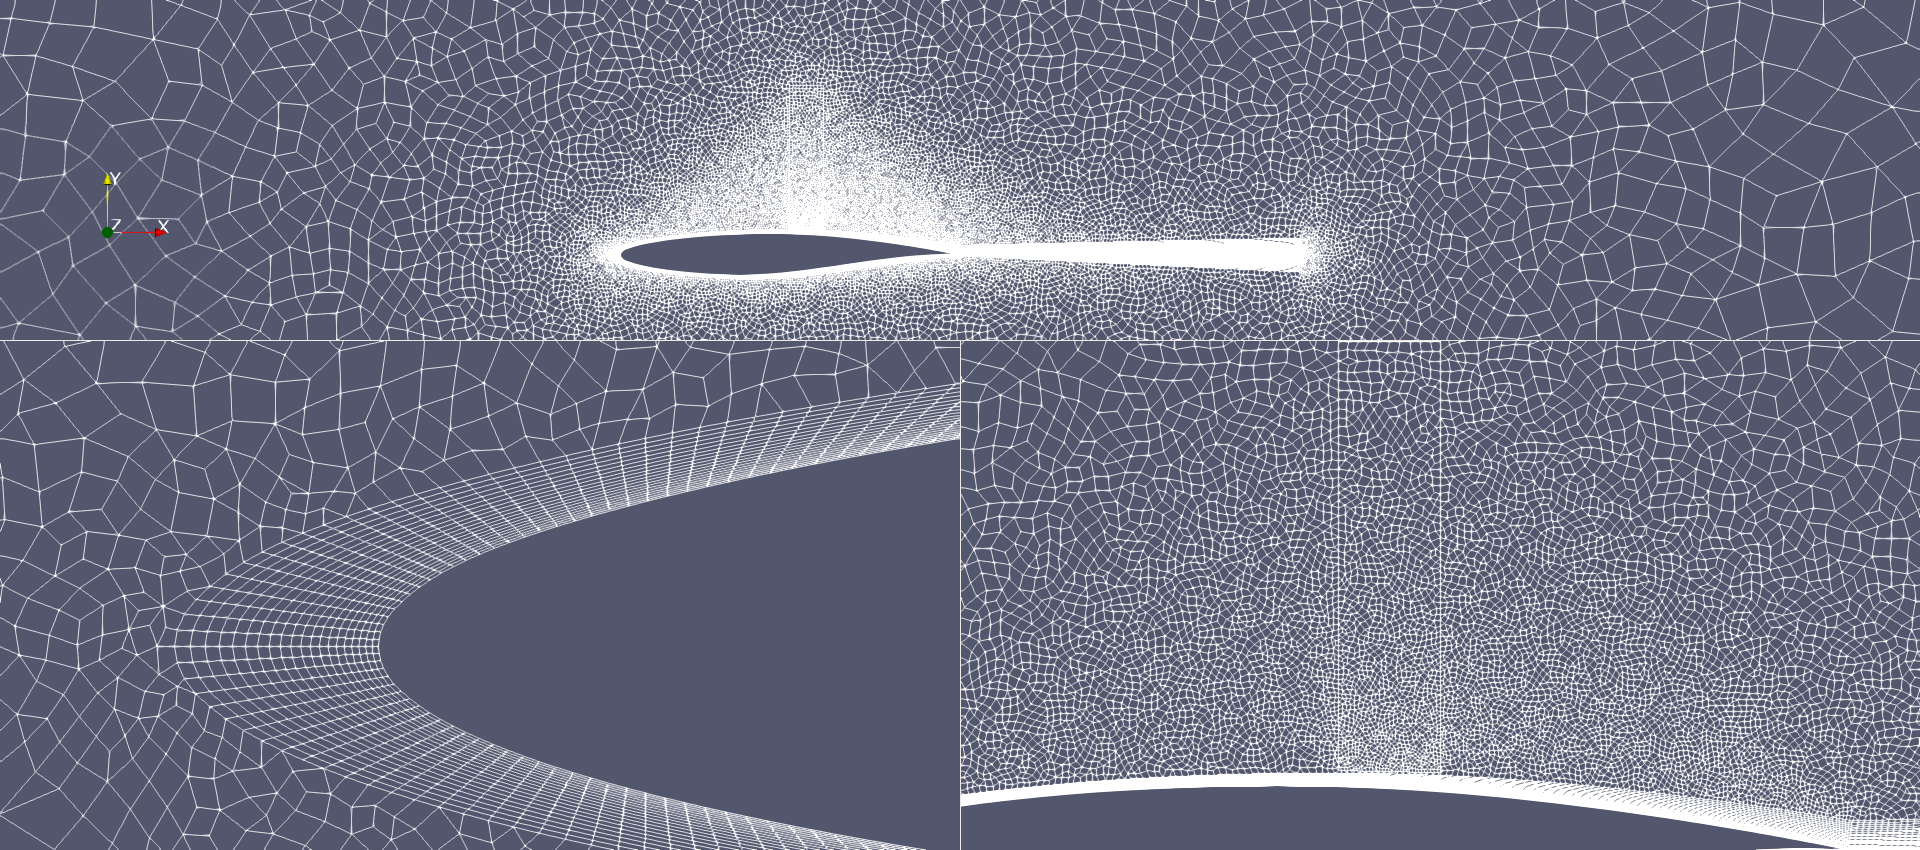
\includegraphics[width=\textwidth]{figures/rae_mesh.png}
          \caption{Mesh for the RAE 2822 test case. Close up on the expected shock location and the wall on the leading edge.}
          \label{fig:rae_mesh}
        \end{figure}

        \paragraph{}
        The model used is the Reynolds Averaged Navier--Stokes equations, or RANS.
        Simply put, every scale of the turbulence is modelled \PS{c'est bien ça ?}.
        For this case, we decided to use the famous Spalart--Allmaras turbulence model.
        It is well known for being one of the simplest turbulence models, which is fine for us as we want to set up a simple first test case.
        The spatial discretisation method is a second-order Finite Volume method, using the HLLC Riemann solver and Multislope method with a Van--Leer slope limiter.
        We also use local time stepping to speed up the convergence.


      \subsubsection{Analysis of the results}

        \PS{Figure champ (mach)}

        \PS{Figure CP comparative}

        \PS{Qu'est-ce qu'on peut regarder pour avoir une différence, flux de chaleur ?}

        \paragraph{}
        We are now going to compare the results from the two different simulations.
        It is first worth noting that before trying the JFNK method, we need to start the computation using the traditional method.
        We assume that because of the matrix-free approximation, it is less robust at the beginning.
        Only some iterations are needed, to start the no slip boundary layer for instance.
        After that, we can restart the computation with the traditional method on one side and with the new method on the other.

        \paragraph{}
        We can first look at a global image of the flow.
        This is done in figure \PS{TODO} where we can look at the pressure field near the airfoil.
        In particular, we see the shock on the upper part, as expected.
        The two computations give similar results: they are indistinguishable by just looking at the pressure field.
        This is to be expected as the traditional method gives already satisfying results on such cases.
        We can also look at the pressure coefficient around the airfoil in figure \PS{TODO}.
        Once again, the two curves are indistinguishable.
        Finally, we can look at the aerodynamic coefficients, the drag and lift coefficients, throughout the simulation on figure \PS{TODO}.
        This time, we see an improvement from our method: the coefficients are much more stable, which mean the convergence is better with out method.

        \paragraph{}
        In order to find out if our method did help the convergence of the solver, we need to look at the residuals.
        To define the residuals, we need to go back at the partial differential equation (\ref{eq:pde}) from which we started.
        The residual is in fact the value of the function $\operatorname{F}$ from this equation.
        We can then understand its name for steady problems: it is what is left and still needs to be removed to find the steady solution.
        To decide on the convergence of a steady simulation, we look at this residual norm throughout the computational domain $\mathcal{D}$.
        More precisely, we look at this residual component by component.
        For example, the residual 2-norm associated with the $i$th component is:
        \begin{equation}
          \norm[2]{\operatorname{F}_i} = \int_\mathcal{D} \left| \operatorname{F}_i \right| \mathrm{d}v
        \end{equation}
        and the $\infty$-norm is:
        \begin{equation}
          \norm[\infty]{\operatorname{F}_i} = \max_\mathcal{D} \left| \operatorname{F}_i \right|
        \end{equation}
        In this fluid dynamics applications, we can look at the residual norm associated to the conservatives variables: the density, the momentum components, the energy and the turbulent variable from the Spalart--Allmaras model $\nu_t$.

        \paragraph{}
        Figure \PS{TODO} shows the residual norms from our two computations.
        The gain from using the JFNK method appears clearly.
        The final residual norm is much smaller for each and every conservative components.
        This means that the Jacobian free Newton--Krylov method is able to reach a better convergence level than the traditional method.
        In other words, the better Jacobian matrix approximation from our new method leads to a better convergence than the older poor approximation.
        \PS{Que dire de plus ?}

        \paragraph{}
        On this first test case, we looked at the residual norms as the fields computed by both methods were almost identical.
        Moreover, our method was even able to reach better convergence levels.
        This validates our method on a first simple case, albeit with turbulence modelling and a shock.


    \subsection{Sphère hypersonique}


  \section{Utilisation de la formulation sans matrice sur un nouveau modèle de fluide}
    \subsection{Modèle Multi-températures}
    \subsection{Sphère hypersonique}
      \subsubsection{Modèle réactif complet}
      \subsubsection{Modèle réactif simplifié}
